\documentclass[a4paper]{article}

% \VignetteIndexEntry{A R package for performing Graphical tests for Hardy-Weinberg Equilibrium}
% \VignetteDepends{graphics,stats}
% \VignetteKeyword{aplot}

% Documentation for the HardyWeinberg package
%
% Note: run first Precalib.R before using Sweave.


\usepackage[english]{babel}
\usepackage{Sweave}
\usepackage{Rd}
\usepackage{url}
\usepackage{hyperref}

\setlength{\parindent}{0cm}

\begin{document}

\input{/graffel/latex/defs}

\begin{center}
\sf
{\sf \bf \Large The {\tt HardyWeinberg} Package}\\
%\normalsize
\vspace{4mm}
{\bf \large Jan Graffelman}\\
\vspace{4mm} \rm \large
Department of Statistics and Operations Research\\
Universitat Polit\`ecnica de Catalunya\\
Avinguda Diagonal 647, 08028 Barcelona, Spain.\\
{\it email:} jan.graffelman@upc.edu\\
\vspace{4mm}
{\sc September 2007}
\end{center}

\section{Introduction}

This guide gives some instructions on how to perform graphical significance tests for Hardy-Weinberg
equilibrium (HWE) by depicting the acceptance region for HWE in a ternary plot with routines from
the package {\tt HardyWeinberg}. The outline of this guide is as follows. Section~2 
describes how the R package {\tt HardyWeinberg} can be installed. Section~3 shows 
how to perform some of the classical tests for Hardy-Weinberg equilibrium with routines from the package. 
Finally, Section~4 shows how to contruct ternary plots with the HW acceptance region 
and how to perform graphical tests for HWE. We refer to Graffelman \& Morales~(2007) 
for the theoretical foundation of the graphical tests. If you appreciate this software then please 
cite the following paper in your work:\\

Graffelman, J. \& Morales-Camarena, J. (2008) Graphical tests for Hardy-Weinberg equilibrium
based on the ternary plot. {\it Human Heredity} {\bf 65}(2): 77-84. 
\special{html:<a href="http://dx.doi.org/10.1159/000108939"}(clic here to access the paper)\special{html:</a>}

\section{Installation}
\label{sec:install}

Packages in R can be installed inside the program with the option "Packages"
in the main menu and then choosing "Install package" and picking the package
"HardyWeinberg". Typing:

\begin{Schunk}
\begin{Sinput}
> library(HardyWeinberg)
\end{Sinput}
\end{Schunk}

will make the functions {\tt HWTernaryPlot, HWChisq, HWLratio} available. 

\section{Classical tests for Hardy-Weinberg equilibrium}
\label{sec:classical}

We show how to perform several classical tests for Hardy-Weinberg equilibrium. As an example we
use a sample of 1000 individuals genotyped for the MN blood group locus described by
Hedrick~(2005, Table 2.4). We store the genotypic counts (298, 489 and 213 for MM, MN and NN
respectively) in a vector {\tt x}:

\begin{Schunk}
\begin{Sinput}
> x <- c(298, 489, 213)
> HW.test <- HWChisq(x, verbose = TRUE)
\end{Sinput}
\begin{Soutput}
Chi2 =  0.2214896 p-value =  0.6379073 D =  -3.69375 
\end{Soutput}
\end{Schunk}

This shows that the $\chi^2$-statistic has value 0.2215, and that the corresponding p-value for 
the test is 0.6379. Taking a significance level of $\alpha = 0.05$, we do not reject HWE for
the MN locus. When {\tt verbose} is set to {\tt FALSE} (default) the test is silent, and {\tt HW.test}
is a list containg the results of the test ($\chi^2$-statistic, the p-value of the test, half the deviation from 
HWE ({\tt D}) for the heterozygote ($D = \frac{1}{2} (f_{AB} - e_{AB}$)) 
and the allele frequency ({\tt p}) of M).

\begin{Schunk}
\begin{Sinput}
> HW.test <- HWChisq(x)
> print(HW.test)
\end{Sinput}
\begin{Soutput}
$chisq
[1] 0.2214896

$pval
[1] 0.6379073

$D
[1] -3.69375

$p
[1] 0.5425
\end{Soutput}
\end{Schunk}

The $\chi^2$-test can also be performed with Yates' continuity correction by setting the {\tt cc} parameter:

\begin{Schunk}
\begin{Sinput}
> HW.test <- HWChisq(x, cc = 0.5, verbose = TRUE)
\end{Sinput}
\begin{Soutput}
Chi2 =  0.1789563 p-value =  0.6722717 D =  -3.69375 
\end{Soutput}
\end{Schunk}

This gives a smaller $\chi^2$-statistic and a larger p-value in comparison with the previous test. The likelihood 
ratio test~(Weir, 1996, Chapter 3) for HWE can be performed by typing

\begin{Schunk}
\begin{Sinput}
> HW.lrtest <- HWLratio(x, verbose = TRUE)
\end{Sinput}
\begin{Soutput}
G2 = 0.2214663 p-value = 0.637925 
\end{Soutput}
\end{Schunk}

Note that the $G^2$-statistic and the p-value obtained are very close to the $\chi^2$-statistic
and its p-value. The Fisher exact test for HWE can be performed by using routine {\tt fisher.test}
from the {\tt stats} package. The genotypic counts are re-organized into a $2 \times 2$ table:


\begin{Schunk}
\begin{Sinput}
> m <- matrix(c(x[1], x[2]/2, x[2]/2, x[3]), ncol = 2)
> colnames(m) <- c("M", "N")
> rownames(m) <- c("M", "N")
> print(m)
\end{Sinput}
\begin{Soutput}
      M     N
M 298.0 244.5
N 244.5 213.0
\end{Soutput}
\begin{Sinput}
> fisher.test(m, alternative = "two.sided")
\end{Sinput}
\begin{Soutput}
	Fisher's Exact Test for Count Data

data:  m 
p-value = 0.6555
alternative hypothesis: true odds ratio is not equal to 1 
95 percent confidence interval:
 0.8238894 1.3794978 
sample estimates:
odds ratio 
  1.066071 
\end{Soutput}
\end{Schunk}

The Fisher exact test leads to the same conclusion, we do not reject HWE ({\tt p=0.6555}).
{\tt HWChisq} and {\tt HWLratio} assume that the data are supplied as a vector of genotypic 
counts listed in order (AA,AB,BB). Additional test for HWE may be added to the package in the near future.

\section{Graphical tests for Hardy-Weinberg equilibrium}
\label{sec:graphical}

This section shows how to create ternary plots for a database of marker data (e.g.\ SNPs) and shows
how the depict the acceptance region for HWE in the ternary plot, using different tests. 
An example with simulated data follows below. We obtain $m=100$ markers for $n=100$ individuals
by taking random samples from a multinomial distribution with $\theta_{AA} = p^2, \hspace{1mm} \theta_{AB} = 2pq, 
\hspace{1mm}$ and $\theta_{BB} = q^2$. The samples are collected in $100 \times 3$ matrix {\tt Xt}, and each sample
is re-expressed as a genotypic composition ({\tt Xc}) with the relative frequencies of AA, AB and BB.

\begin{Schunk}
\begin{Sinput}
> set.seed(123)
> nm <- 100
> Xt <- NULL
> for (i in 1:nm) {
+     p <- runif(1)
+     X <- t(rmultinom(1, size = 100, prob = c(p^2, 2 * p * (1 - 
+         p), (1 - p)^2)))
+     Xt <- rbind(Xt, X)
+ }
> Xc <- Xt/100
> colnames(Xt) <- c("AA", "AB", "BB")
> colnames(Xc) <- c("AA", "AB", "BB")
\end{Sinput}
\end{Schunk}

We create four different ternary plots for the simulated marker data shown in Figure~1. Panel
(a) simply depicts the 100 genotypic compositions in a ternary plot. Note the marked curvature
in the cloud of points. Panel (b) shows a nicer ternary plot with the HWE curve and the acceptance region 
for HWE according to an ordinary $\chi^2$-test. Green markers are not significant, red markers significant 
($\alpha = 0.05$). 6 markers show up significant. Panel (c) shows the same data, but the acceptance region 
represented corresponds
to a $\chi^2$-test with continuity correction ({\tt cc = 0.5}), with separate curves for $D>0$ and $D<0$. 
Some markers previously significant markers now turn
up insignificant. Panel (d) shows the acceptance region for Fisher's exact test. This option takes
more computer time. The significant markers are the same ones that are significant in the $\chi^2$-test with
continuity correction. 
\begin{figure}[htb]
\centering
\begin{Schunk}
\begin{Sinput}
> plot.new()
> opar <- par(mfrow = c(2, 2), mar = c(3, 5, 3, 1) + 0.1, mex = 0.75, 
+     oma = c(2, 0, 2, 0), new = TRUE)
> par(mfg = c(1, 1))
> Res <- HWTernaryPlot(Xc, 100, region = 0, hwcurve = FALSE, vbounds = FALSE, 
+     vertex.cex = 1.25, main = "(a)")
> par(mfg = c(1, 2))
> Res <- HWTernaryPlot(Xc, 100, region = 1, vertex.cex = 1.25, 
+     signifcolour = TRUE, main = "(b)")
> par(mfg = c(2, 1))
> Res <- HWTernaryPlot(Xc, 100, region = 2, vertex.cex = 1.25, 
+     signifcolour = TRUE, main = "(c)")
> par(mfg = c(2, 2))
> Res <- HWTernaryPlot(Xc, 100, region = 7, vertex.cex = 1.25, 
+     signifcolour = TRUE, main = "(d)")
> par(opar)
\end{Sinput}
\end{Schunk}
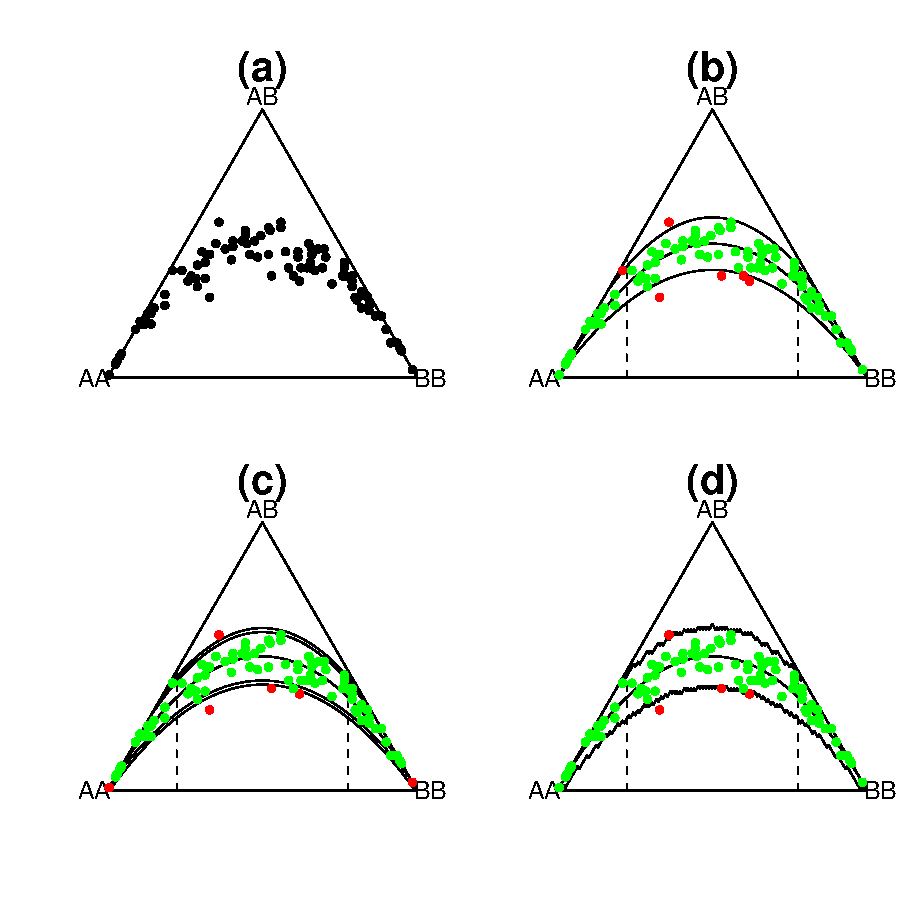
\includegraphics{HardyWeinberg-008}
\caption{Ternary plot of 100 simulated SNPs for 100 individuals. (a): ordinary ternary plot, (b): with $\chi^2$-acceptance
region, (c) with acceptance region for $\chi^2$-test with continuity correction, (d): with acceptance region for two-tailed
FE test.}
\end{figure}
More examples with human SNP data are given in Graffelman \& Morales~(2008).

\clearpage

\section{Online documentation}
\label{sec:online}

The online documentation for the most important routines of the package is
included below.

\include{/graffel/latex/HWChisq}

\include{/graffel/latex/HWLratio}

\include{/graffel/latex/HWTernaryPlot}

%\url{http://www-eio.upc.es/}

\section*{Acknowledgements}

This work was partially supported by the Spanish grant SEJ2006-13537 This document was generated by 
Sweave~(Leisch, 2002).

\section{References}

Graffelman, J. \& Morales-Camarena, J. (2008) Graphical tests for Hardy-Weinberg equilibrium
based on the ternary plot. {\it Human Heredity} {\bf 65}(2): 77-84.\\

Hedrick, P. W. (2005) Genetics of Populations. Third edition. Jones and Bartlett Publishers,
Sudbury, Massachusetts.\\

Weir, B. S. (1996) Genetic Data Analysis II. Sinauer Associates, Massachusetts.

\end{document}
